\documentclass[30pt,margin=1in,innermargin=-4.5in,blockverticalspace=-0.25in]{tikzposter}
\geometry{paperwidth=33.11in,paperheight=46.81in} %A0
% \geometry{paperheight=33.11in,paperwidth=23.4in} %A1
\usepackage[utf8]{inputenc}
\usepackage{csquotes}
%\usepackage[estonian]{babel}
\usepackage{amsmath}
\usepackage{amsfonts}
\usepackage{amsthm}
\usepackage{amssymb}
\usepackage{mathrsfs}
\usepackage{graphicx}
\usepackage{lipsum}
\usepackage[export]{adjustbox}
\usepackage{enumitem}
\usepackage[backend=biber,style=numeric]{biblatex}
\usepackage{unitartu-theme}
\makeatletter
\setlength{\TP@visibletextwidth}{31.0in}
\setlength{ \TP@visibletextheight}{45in}
\makeatother
\usepackage{mwe} % for placeholder images
\usepackage{bm}
\usepackage{bbm}

\addbibresource{refs.bib}

% set theme parameters
\tikzposterlatexaffectionproofoff
\usetheme{UniTartuTheme}
\usecolorstyle{UniTartuStyle}

\usepackage[scaled]{helvet}
\renewcommand\familydefault{\sfdefault} 
\renewcommand{\vec}[1]{\bm{#1}}
\newcommand{\Tr}{\text{Tr}}
\usepackage[T1]{fontenc}


\title{\parbox{0.8\linewidth}{A Distributed and Scalable Order Fulfillment Architecture for E-Commerce Platforms}}
\author{\textbf{Ronald Judin}\textsuperscript{1} \textbf{Kalju Jake Nekvasil}\textsuperscript{1}}
\institute{\textsuperscript{1}Institute of Computer Science, University of Tartu}

\titlegraphic{
\includegraphics[width=0.35\linewidth]{unitartu_compact.png}}

% begin document
\begin{document}
\maketitle
\centering
\begin{columns}
    \column{0.5}
    \block{Introduction}{
       We propose a distributed order fulfillment architecture designed for high-throughput e-commerce platforms. Modern online retailers like Amazon need reliability during traffic spikes and consistency for concurrent orders. Our system addresses these with orchestrated parallel verification, priority-based task queuing, and fault-tolerant two-phase commits for payments and shipping.
	}

    \block{System Model}{
The system follows a distributed orchestration model. A client submits an order to the orchestrator, which initiates multithreaded parallel calls to the identity and inventory services. These services perform READ requests against the leader database to validate the request. After receiving APPROVED responses from both services, the orchestrator adds the order to a priority queue. Auto-scaling executors then process orders from the queue, coordinating two-phase commit (2PC) transactions with the shipping and payment services which guarantees ACID compliance for writes. After both services acknowledge (ACK) the Commit phase, the executor dequeues the order and triggers the notification service to inform the user. Throughout this workflow, the analytics service asynchronously logs requests, errors, and metrics for observability. The design prioritizes scalability (with auto-scaling and multithreading), consistency (with 2PC and leader DB reads), and fault tolerance (with queue-based retries and analytics monitoring).


       \begin{align*}
            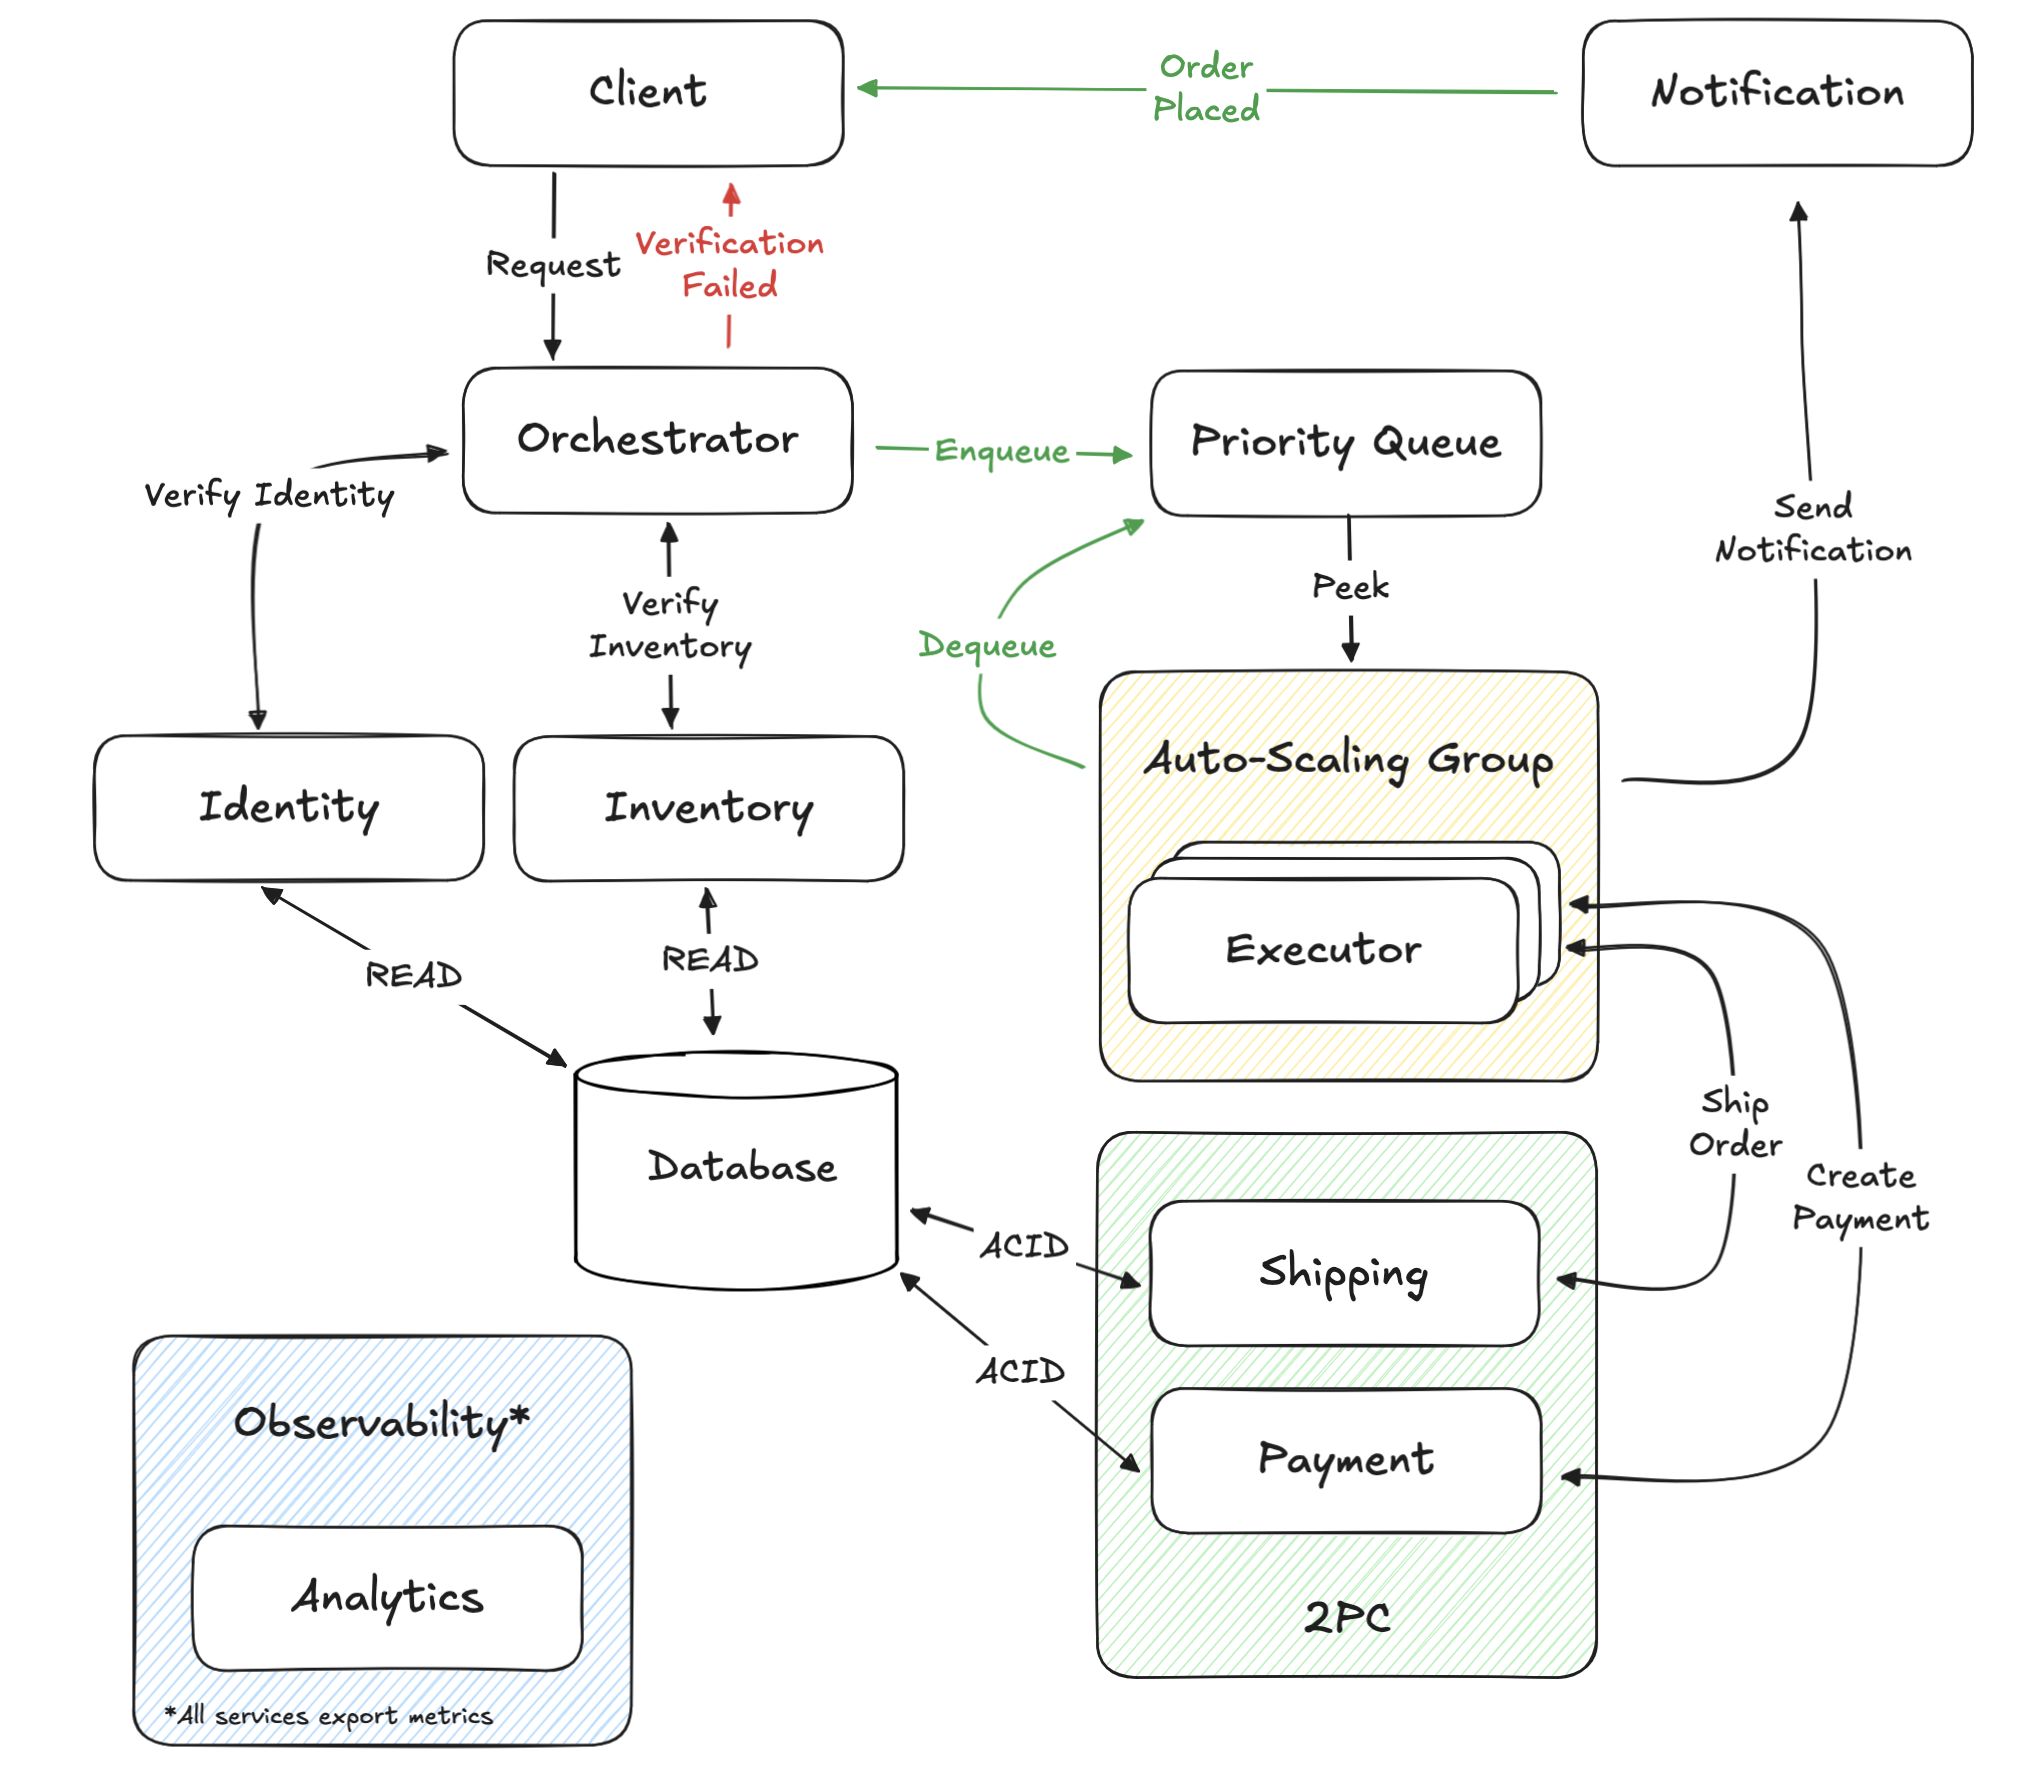
\includegraphics[width=0.5\textwidth,valign=c]{system_diagram}
        \end{align*}
    }
    
 
    

            \block{Replication}{

Two types of replication are used in our distributed system. The executor service uses queue-based replication. The auto-scaling executors are stateless and rely on the priority queue for order assignment. Unlike database replication, orders persist in the queue until successfully processed (durable) and executors scale dynamically based on queue size (elastic). The database uses a synchronous leader-follower replication. The leader handles all writes and the followers serve read requests. This behavior allows for strong consistency (followers mirror leader state before acknowledging reads) and fault tolerance (automatic elections during leader replica failure minimizes database downtime).

       		\begin{align*}
        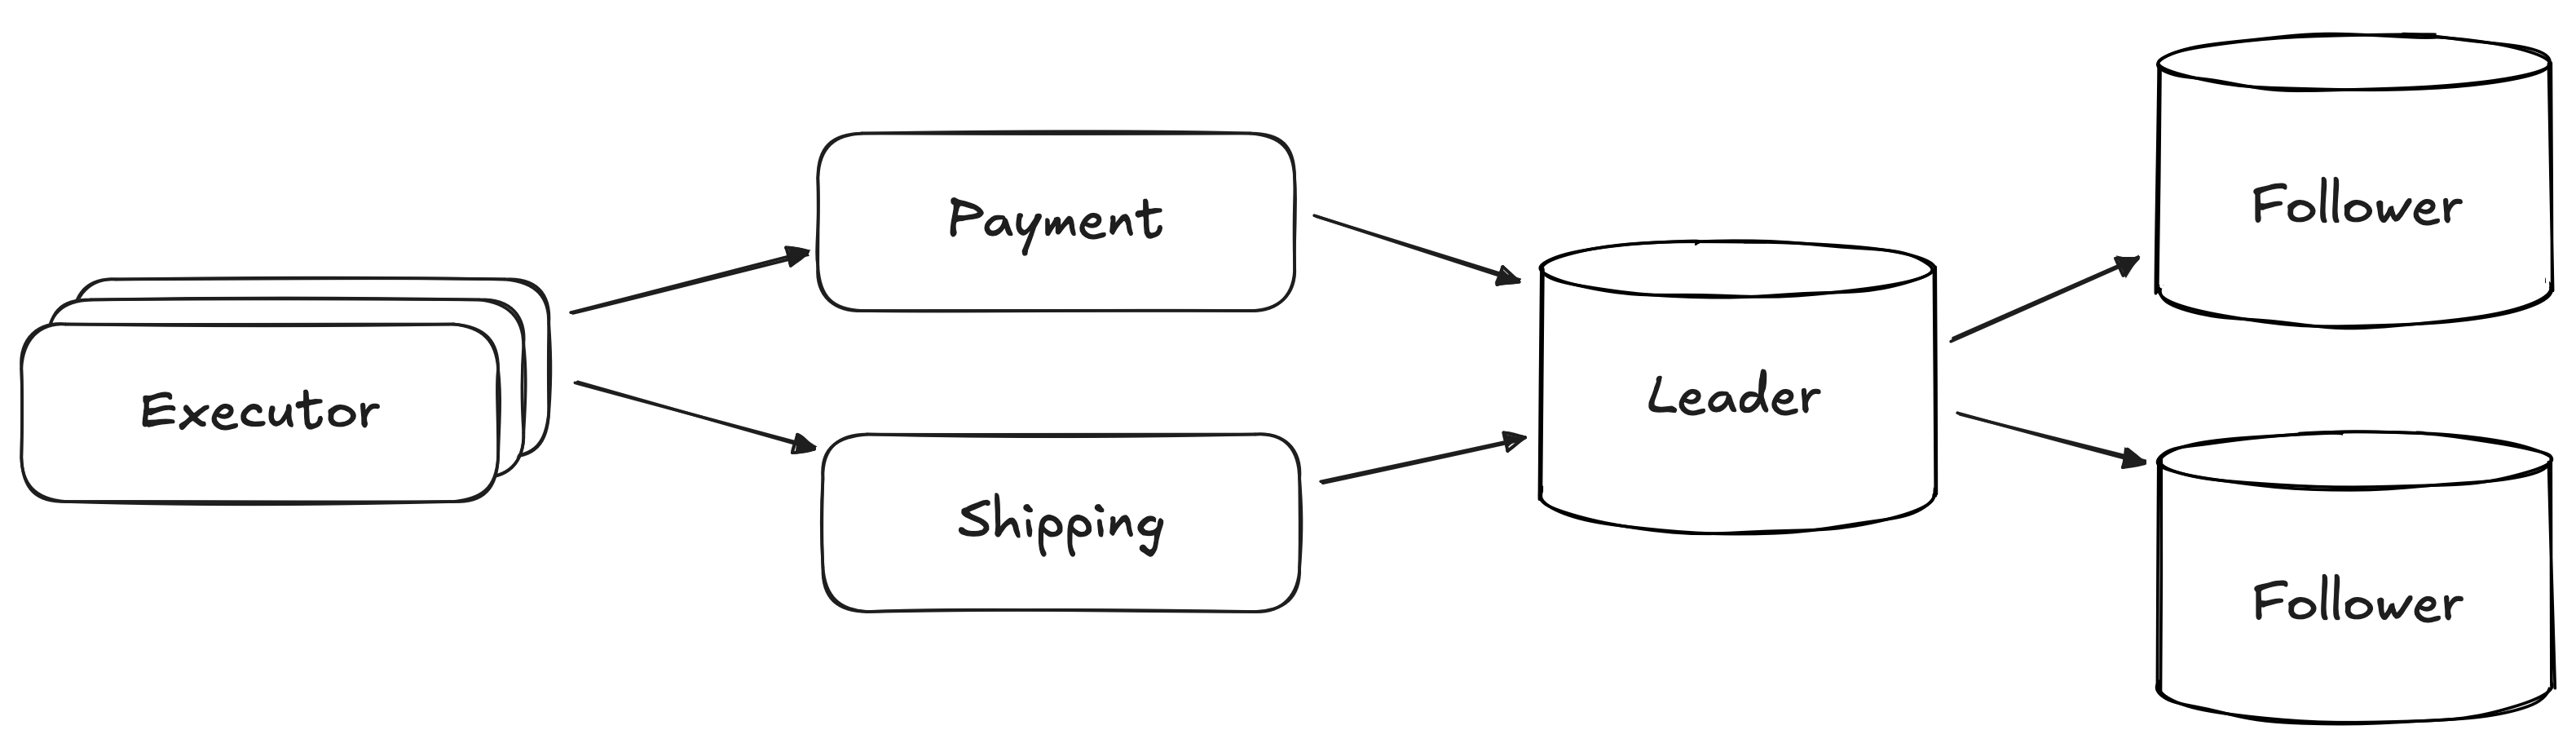
\includegraphics[width=0.45\textwidth,valign=c]{db_replication}
        \end{align*}
    }



    \column{0.5}
   \block{Vector Clocks}{
The analytics service uses vector clocks to track causal relationships between events across the entire workflow from order request to placement. This tracking can be used for monitoring race conditions in real-time and debugging in the future. Below shows the general expected vector clock tracking timeline. For readability purposes, we do not display the vector value at every event.
 		\begin{align*}
        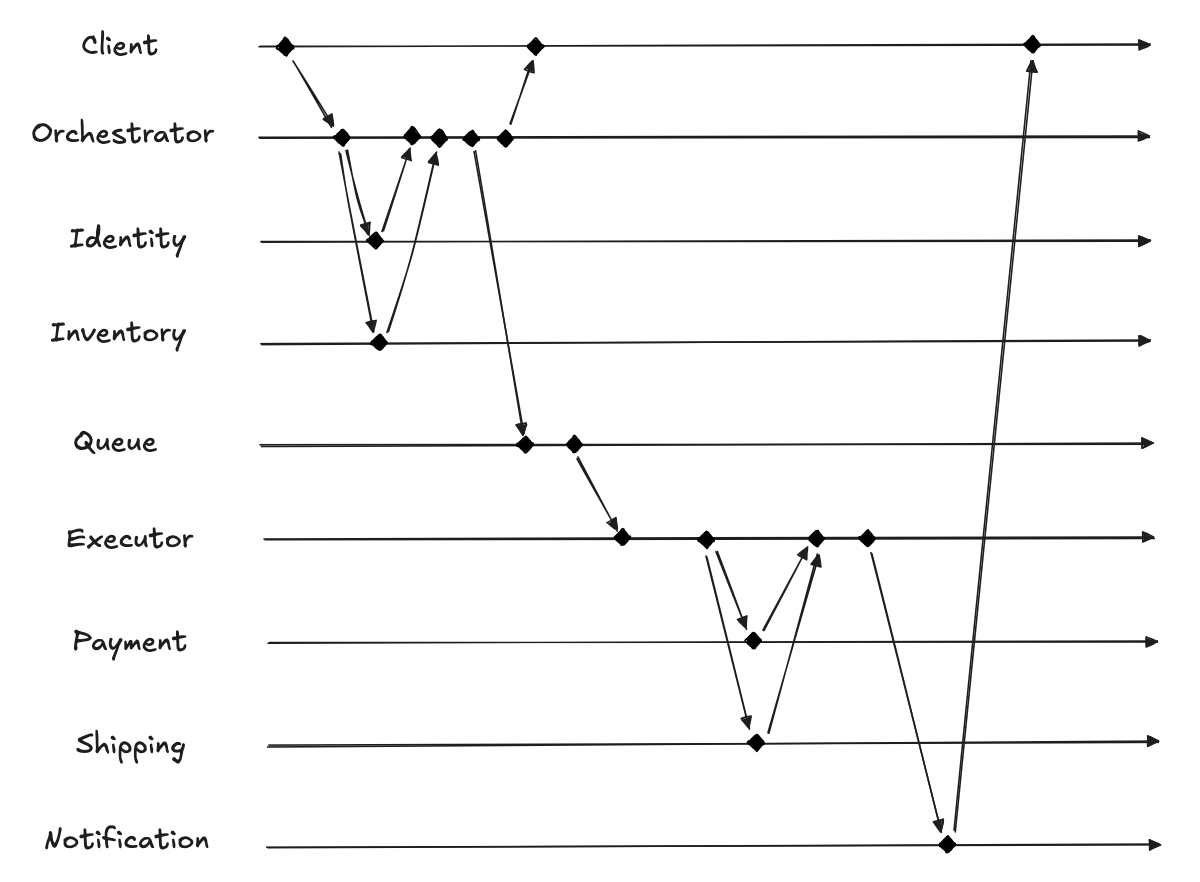
\includegraphics[width=0.5\textwidth,valign=c]{vector_clock}
        \end{align*}
    }

        \block{Commitment Protocol}{
    
The system uses two-phase commit (2PC) between the executor, payment, and shipping service to ensure atomic order processing. To handle failures, the system uses optimistic exponential backoff retries. If retries breach a set threshold, the analytics service can be used to track all logs, errors, and other specific order failure information.
    
   		\begin{align*}
        	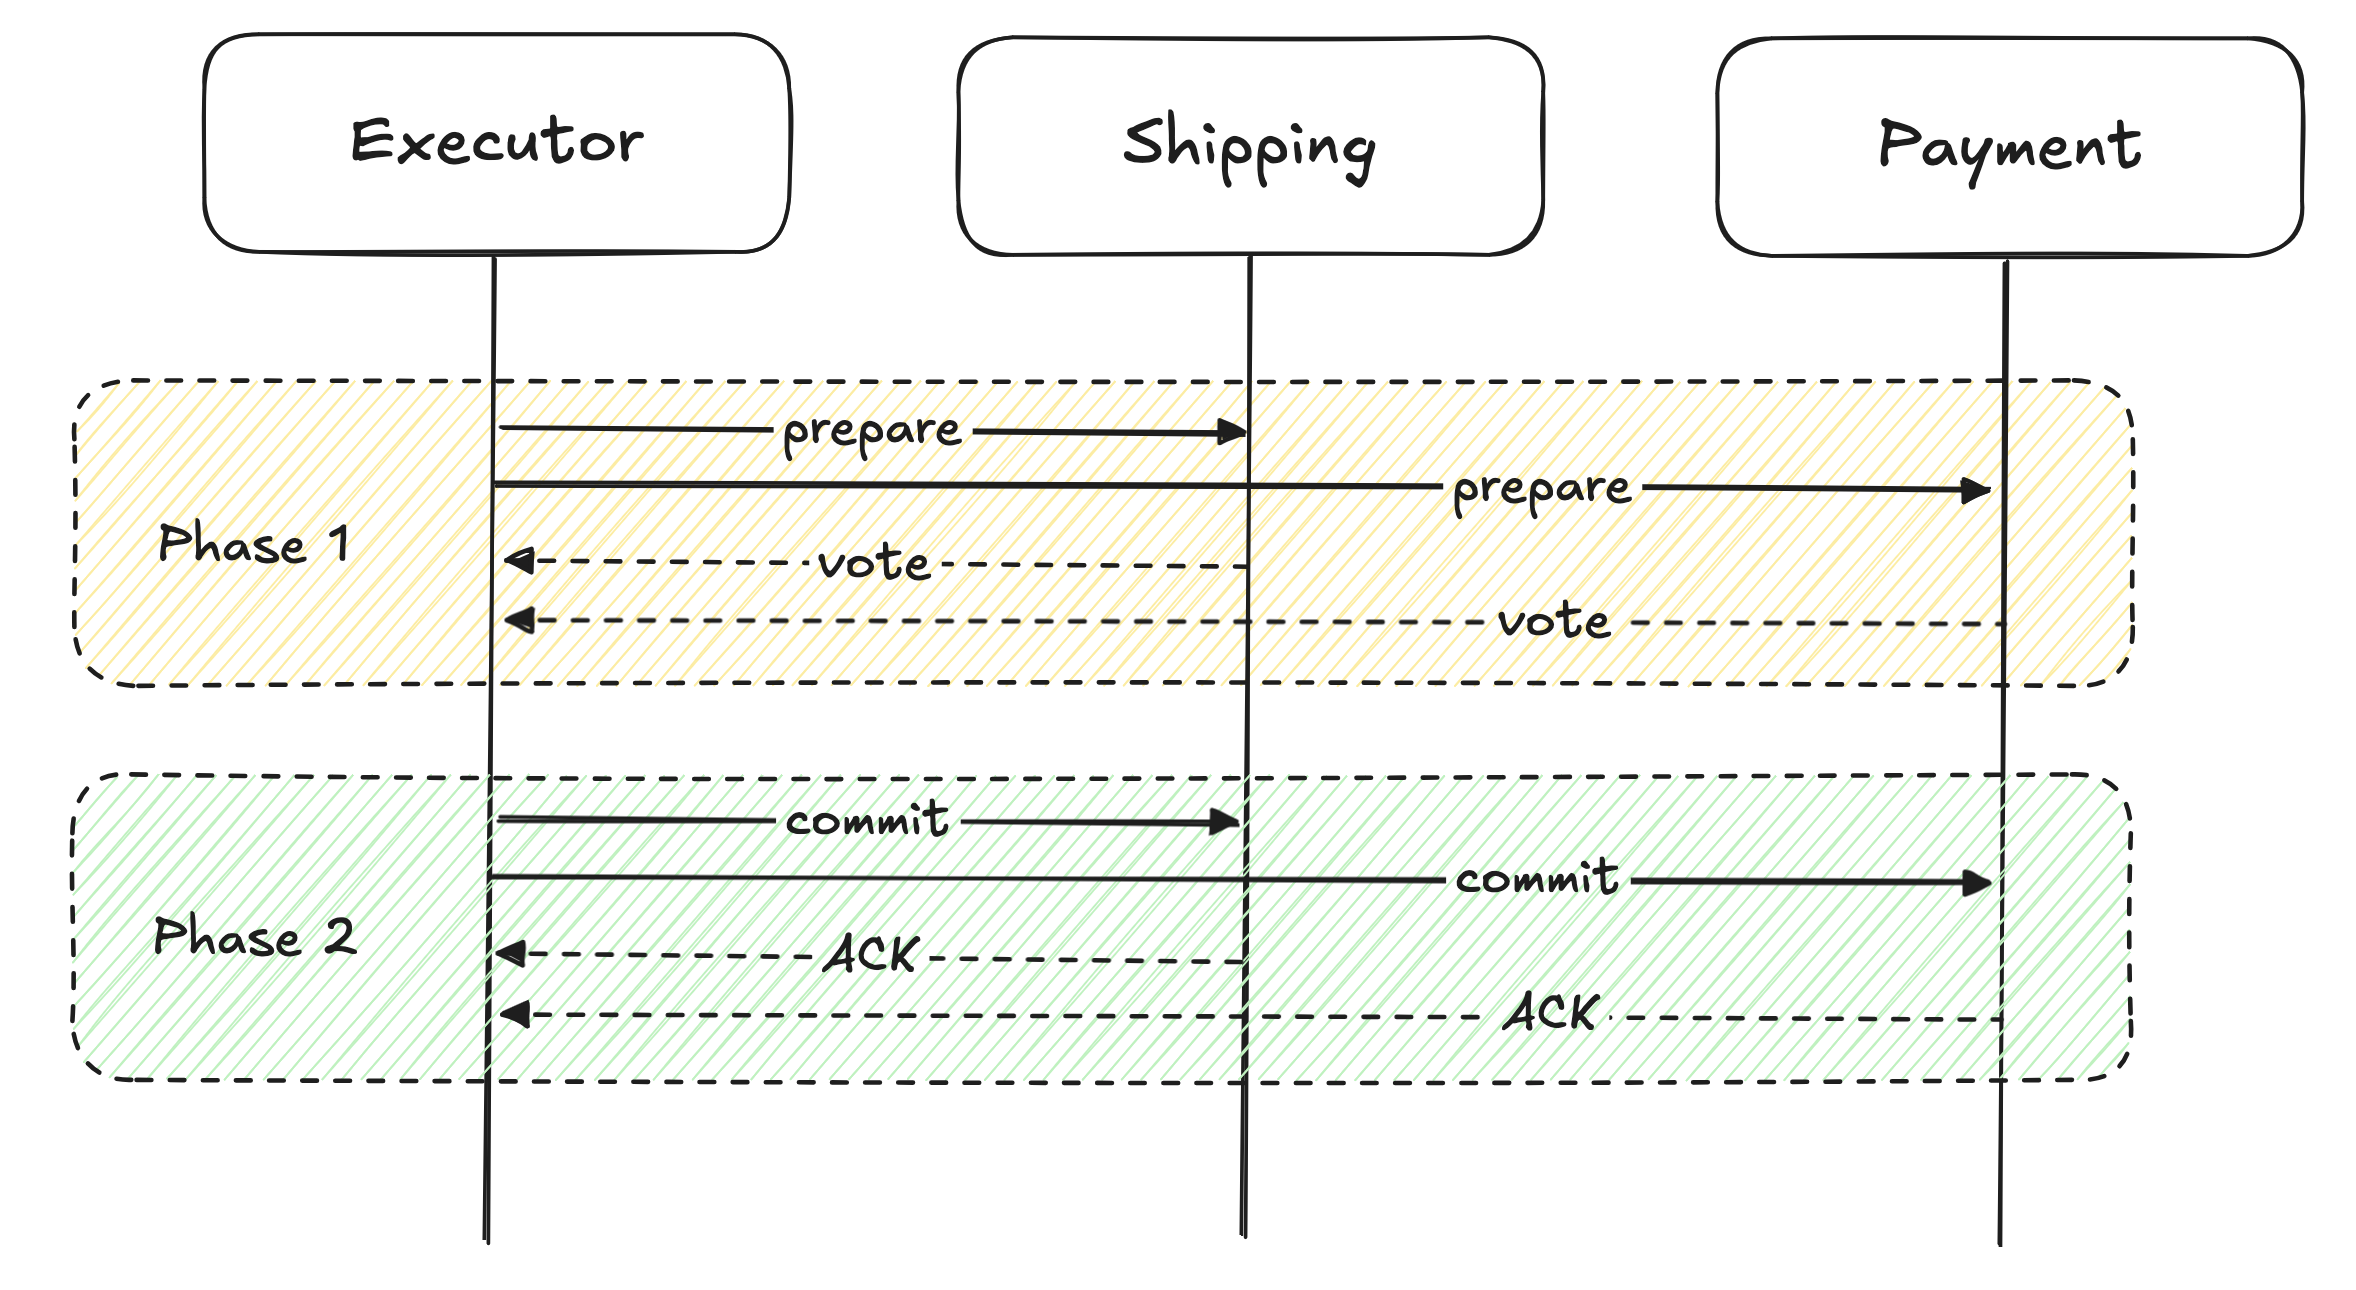
\includegraphics[width=0.48\textwidth,valign=c]{consensus}
        \end{align*}

    }
    
    
\block{Conclusion}{
    This distributed order fulfillment system executes reliable e-commerce processing through orchestrated parallel verification, priority-based queuing, and fault-tolerant 2PC transactions. The architecture coordinates between stateless executors, strongly-consistent database replication, and broad service monitoring to achieve scalable, consistent order processing.}
\end{columns}
\end{document}